\documentclass[aspectratio=169]{beamer}
\usetheme{Uppsala}
\usepackage[caption=false]{subfig}
\usepackage[]{graphicx}
\usepackage{tikz}
\usepackage[]{physics}
\usepackage[bb=dsserif]{mathalpha}
\usepackage[english]{babel}
\newcommand{\R}{\ensuremath{\mathbb{R}}}
\newcommand{\C}{\ensuremath{\mathbb{C}}}
\newcommand{\Arg}{\ensuremath{\text{Arg}}}
\newcommand{\U}{\ensuremath{\mathbb{\cal U}}}
\renewcommand{\va}{\vec}

\usetikzlibrary{arrows.meta}
\usetikzlibrary{decorations.pathreplacing}
\usetikzlibrary{decorations.markings}
\usetikzlibrary{patterns}
\usetikzlibrary{3d}
\usetikzlibrary{math}
\usetikzlibrary{calc}

\newcommand\blfootnote[1]{%
\begingroup
\renewcommand\thefootnote{}\footnote{#1}%
\addtocounter{footnote}{-1}%
\endgroup
}

\newenvironment{psmallmatrix}
    {\left(\begin{smallmatrix}}
    {\end{smallmatrix}\right)}

\author[Ola Carlsson]{Ola Carlsson \\ Supervisor: Erik
Sjöqvist \\ Subject reviewer: Patrik Thunström}
\title{Simulating classical motion in synthetic monopole fields}
\subtitle{Bachelor's thesis  15 credits}
\date[\today]{\today}
\institute[Department for Physics and Astronomy]{Department for Physics and Astronomy, division of Materials Theory}

\begin{document}
%% For the title
\begin{frame}[plain]
  \titlepage
\end{frame}
\section{Introduction and premise}
\begin{frame}
  \frametitle{Magnetic monopoles}
  \begin{itemize}
          \item The Maxwellian M-field does not display
                  monopoles.
          \item Non-fundamental or non-Maxwellian monopoles do however appear in nature.
          \item A particular example are the synthetic magnetic monopoles generating the
                  geometrical phase.
          \item These synthetic monopoles sit in parameter space, presently the space of
                  external magnetic fields, at points of energy
                  degeneration.
  \end{itemize}
\end{frame}
\begin{frame}
    \frametitle{Stranger field textures}
        \begin{itemize}
                \item Multipartite spin systems complicate the situation first explored by
                        Berry, splitting the monopoles to positions away from the
                        origin.\footnote{A. Eriksson and E. Sjöqvist, “Monopole field textures in interacting spin systems”, Physical Review A
101 (2020).}
            \item In addition the synthetic field texture then displays nonzero curl, i.e.
                    we can define a synthetic "current" to complete the analogy with
                    Maxwellian fields.
            \item How does such an exotic magnetic field structure affect our world, i.e.
                    what dynamics result?
            \item To this end a specific bipartite system displaying desired properties was modelled
                    and simulated.
        \end{itemize}
\end{frame}
\section{System description}
\subsection{The dumbbell}
\begin{frame}
        \frametitle{The dumbbell system}
        \begin{columns}
            \begin{column}{.49\textwidth}
                \begin{itemize}
                    \item Two masses each carrying spin-\(\frac{1}{2}\) with fixed distance to another were considered in translation and rotation ---the ''dumbbell''.
                    \item An external magnetic field is present.
                    \item \(\mathbb{\cal H} = \sum_{i=1}^{5} \frac{\va{p_i}^2}{2m_i} +
        \frac{4J}{\hbar{}}S^{(1)}_{\mu}S^{(2)}_{\mu} -
        \gamma\va{B}\cdot \va{S}.\)
                \end{itemize}
            \end{column}
            \begin{column}{.49\textwidth}
                \begin{figure}
        \begin{tikzpicture}[scale=0.8]
            \draw[black, thick] 
                    node[anchor=north,
                    xshift=-0.5cm]{\huge\(\ket{s, m_1}\)} (0,0) -- (4.9,3.4)
                    node[anchor=south, xshift=0.5cm]{\(\ket{s, m_2}\)};
            \draw[black, thick] (1, -0.3) -- (5,3.4);
            \draw[blue, thick, postaction=decorate, decoration={pre length = 1mm, post length = 1mm, markings, mark=
                        between positions 0.1 and 1 step
                        0.25 with {\pgftransformscale{2}\arrow{stealth}}}] plot [smooth, tension=1] coordinates {(-1,3.5) (1,1) (4,0)};
            \draw[blue, thick, postaction=decorate, decoration={pre length = 1mm, post length = 1mm, markings, mark=
                        between positions 0.1 and 1 step
                        0.4 with {\pgftransformscale{2}\arrow{stealth}}}] plot [smooth, tension=1] coordinates {(3,3.7) (3.5,2.5) (4.3,1.5)};
            \draw[blue, thick,  postaction=decorate, decoration={pre length = 1mm, post length = 1mm, markings, mark=
                        between positions 0.1 and 1 step
                        0.28 with {\pgftransformscale{2}\arrow{stealth}}}] plot [smooth, tension=1] coordinates {(1,3.6) (2.5,1.5) (4.2,0.8)};
            \draw[blue] (4.2,0.8) node[anchor=west, xshift=0cm]{\huge\(\va{B}\) };
        \end{tikzpicture}
                \end{figure}
 %\includegraphics[\textwidth]{fig}
 \end{column}
\end{columns}
\end{frame}
\begin{frame}
        \begin{itemize}
                \item{ Effective masses: \(
        m_i = \begin{cases}
                m, & i = 1, 2, 3,\\
                \frac{ml^2}{4}, & i = 4, 5.
        \end{cases}
\)}
\item Matrix forms of the spin operators must be rotated according to the dumbbell and
        external field, \(
        \U_{m'm''} = \bra{s,
        m'}e^{\frac{-iS_\mu\alpha}{\hbar}}e^{\frac{-iS_y\beta}{\hbar}}e^{\frac{-iS_\mu\delta}{\hbar{}}}\ket{s,
m''}\)
  \(\frac{\va{B}\cdot \va{S}}{B\hbar{}} =
        \begin{psmallmatrix}
                0& & & \\
                 &-1 & & \\
                 & & 0 &\\
                 & & & &1
        \end{psmallmatrix} \to \begin{psmallmatrix}
            0 & 0 & 0 & 0\\
            0 & -\cos(\vartheta_B) & \frac{e^{-i\varphi_B}}{\sqrt{2} }\sin(\vartheta_B) & 0\\
                    0 & \frac{e^{i\varphi_B}}{\sqrt{2} }\sin(\vartheta_B) & 0 &
                    \frac{e^{-i\varphi_B}}{\sqrt{2} }\sin(\vartheta_B)\\
                    0 & 0 & \frac{e^{i\varphi_B}}{\sqrt{2} }\sin(\vartheta_B) &
                    \cos(\vartheta_B)\end{psmallmatrix}
\)

\(4\frac{S^{(1)}_\mu S^{(2)}_\mu}{\hbar{}^{2}} =
        \begin{psmallmatrix} 
        -1& & & \\
         &1& & \\
         & &-1& \\
         & & &1
        \end{psmallmatrix}
        \to 
        \begin{psmallmatrix}-1 & 0 & 0 & 0\\
                0 & \cos[2](\vartheta_r) & -\frac{e^{i\varphi_r}}{\sqrt{2}
                }\sin(2\vartheta_r) & e^{-2i\varphi_r}\sin[2](\vartheta_r)\\
                0 & -\frac{e^{-i\varphi_r}}{\sqrt{2}
                }\sin(2\vartheta_r) & -\cos(2\vartheta_r) & \frac{e^{-i\varphi_r}}{\sqrt{2}
        }\sin(2\vartheta_r)\\
        0 & e^{2i\varphi_r}\sin[2](\vartheta_r) & \frac{e^{i\varphi_r}}{\sqrt{2}
        }\sin(2\vartheta_r) & \cos[2](\vartheta_r)
        \end{psmallmatrix}
        \)
        \end{itemize}
\end{frame}
\subsection{Born-Oppenheimer approximation}
\begin{frame}
\frametitle{The Born-Oppenheimer approximation}
\begin{itemize}
        \item The Hamiltonian is heavily coupled and not easily solvable
        \item The Born-Oppenheimer approximation assumes parametrisation of ''fast''
                subsystem by ''slow'' subsystem.
        \item \(\ket{\Psi_{full}} = \Psi_s\ket{n}\)
        \item \(\mathbb{\cal H}_f \ket{n} = E_n\ket{n}\)
        \item \(\mathbb{\cal H}_s = \sum_{n=1}^{5} \frac{p_i^2}{2m_i}\)
        \item Effective Hamiltonian for the slow subsystem (system coordinates) is governed
                by an effective Hamiltonian \(\mathbb{\cal H}^{(n)}_{eff} =
\bra{n}\mathbb{\cal H}_s\ket{n} + E_n\)
\end{itemize}\end{frame}
\begin{frame}
        \frametitle{Synthetic fields}
        \begin{itemize}
                \item Manipulation yields 
\begin{align}
        \mathbb{\cal H}^{(n)}_{eff} &= \sum_{i=5}^{5} \frac{(p_i - A^{(n)}_i)^2}{2m_i} + \Phi^{(n)} + E_n,\\
        A^{(n)}_i &= i\hbar{}\bra{n}\ket{\partial_i n},\\
        \Phi^{(n)} &= \sum_{i=1}^{5} \frac{\hbar{}^{2}}{2m_i}\bra{\partial_i n}(\mathbb{1} - \ket{n}
    \bra{n})\ket{\partial_i n}
.\end{align}
\item \(A_i^{(n)}\) is the synthetic magnetic field containing the monopoles.
        \end{itemize}
\end{frame}
\subsection{System solution}
\begin{frame}
        \frametitle{Equations of motion}
        \begin{itemize}
                \item It is now practical, and appropriate, to consider the slow system
                        classical and find the dynamics per Hamilton's Canonical Equations:
                \item \(m\frac{d \va{r}}{d t^2} = \va{F}^A-\frac{\partial \Phi^{(n)}}{\partial
        \va{r}} - \frac{\partial E_n}{\partial \va{r}} \)
                \item \(\frac{1}{i\hbar{}}F_i^A = 2i\sum_{j\ne i} \sum_{l \ne n} \frac{\frac{\partial r_j}{\partial
        t}}{\pqty{E_n-E_l}^2} \Im \bqty{\bra{n}\partial_i \mathbb{\cal H}_f
        \ket{l}\bra{l}\partial_j\mathbb{\cal H}_f\ket{n}}
        \)
\item \(\Phi^{(n)} = \sum_{i=1}^{5} \sum_{l \ne n}
    \frac{\hbar{}^2}{2m_i}\frac{|\bra{n}\partial_i \mathbb{\cal H}_f\ket{l}|^2}{\pqty{E_n-E_l}^2}
    \)
\item The fast Hamiltonian is analytically differentiable.
        \end{itemize}
\end{frame}
\section{Simulation}
\begin{frame}
        \frametitle{Simulation strategy}
        \begin{columns}
                \begin{column}{0.49\textwidth}
        \begin{itemize}
                \item A ''lab'' region was discretized to allow for stored external field
                        values.
                \item Two opposite square coils generate an external field zero at the centre.
                \item Numerical differentiation could benefit from finer lab division.
        \end{itemize}
        \end{column}
        \begin{column}{0.49\textwidth}
        \begin{figure}[h]
                \centering
                \def\dgrid[####1](####2,####3)(####4)(####5)(####6){ %[draw options](corner)(distance in x)
                %(distance in y)(number of lines -1  per side)
                \foreach \x in {0,1,...,####6}{
                        \pgfmathsetmacro\sx{\x*####4/####6}
                        \draw[####1] (####2+\sx,####3) -- (####2+\sx,####3+####5);
                        }
                \foreach \y in {0,1,...,####6}{
                        \pgfmathsetmacro\sy{\y*####5/####6}
                        \draw[####1] (####2,####3+\sy) -- (####2+####4, ####3+\sy);
                        }
                }
                \begin{tikzpicture}[decoration={markings, mark= between positions 0.1 and 1 step
                        0.2 with {\arrow{stealth}}},
                        z={(90:10mm)},x={(-25:6mm)},y={(0:10mm)},
                        scale=0.6]
                    \begin{scope}[canvas is xy plane at z=0]
                        \draw[black, thick, postaction={decorate}] (0,0) -- (6,0) -- (6,6) -- (0,6) -- cycle;
                    \end{scope}
                    \dgrid[red, dotted, thick, canvas is xy plane at z=1](1,1)(4)(4)(8); %Draw the lab
                    \dgrid[red, dotted, thick, canvas is xy plane at z=5](1,1)(4)(4)(8);
                    \dgrid[red, dotted, thick, canvas is yz plane at x=1](1,1)(4)(4)(8);
                    \draw[blue] (3,3,3) node[circle, fill, inner sep=2pt]{}; %Zerofield marker
                    \dgrid[red, dotted, thick, canvas is yz plane at x=5](1,1)(4)(4)(8);
                    \dgrid[red, dotted, thick, canvas is zx plane at y=1](1,1)(4)(4)(8);
                    \dgrid[red, dotted, thick, canvas is zx plane at y=5](1,1)(4)(4)(8);
                    \begin{scope}[canvas is xy plane at z=6]
                        \draw[black, thick, postaction={decorate}] (0,0) -- (0,6)
                                node[anchor=west, xshift=2mm, yshift=2mm]{\Large I} -- (6,6) -- (6,0) -- cycle;
                    \end{scope}
                \end{tikzpicture}
        \end{figure}
        \end{column}
        \end{columns}
\end{frame}

\section{Results}
\subsection{Eigenstates}
\begin{frame}
        \frametitle{Simulations}
    \begin{figure}[h]
        \centering
        \subfloat[\centering \(n =
        0\)]{{\includegraphics[width=3cm]{figures/n_compare/I10nr101lablength0.001tmax0.1J100000.0Gamma10000000000.0mass3.58e-25len5e-05n0vel(0.01,
                0, 0, 0, 0)swarmnum4norotFalsenosynFalse}}}
        \qquad
        \subfloat[\centering \(n = 1\)]{{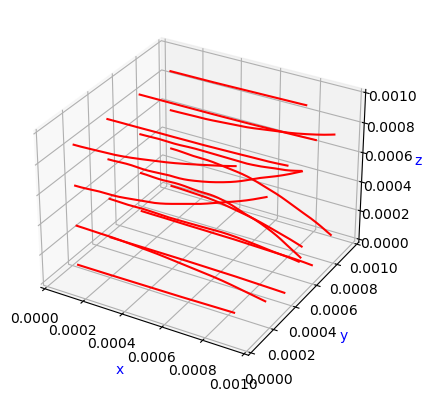
\includegraphics[width=3cm]{figures/n_compare/I10nr101lablength0.001tmax0.1J100000.0Gamma10000000000.0mass3.58e-25len5e-05n1vel(0.01, 0, 0, 0, 0)swarmnum4norotFalsenosynFalse}}}
        \qquad
        \subfloat[\centering \(n = 2\)]{{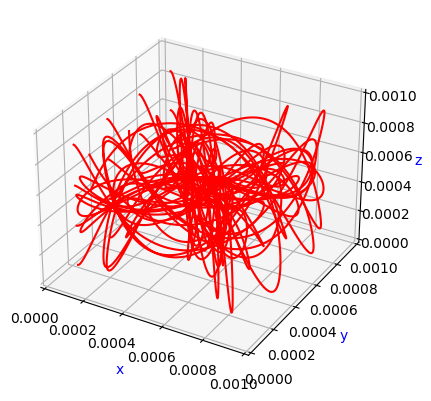
\includegraphics[width=3cm]{figures/n_compare/I10nr101lablength0.001tmax0.1J100000.0Gamma10000000000.0mass3.58e-25len5e-05n2vel(0.01, 0, 0, 0, 0)swarmnum4norotFalsenosynFalse}}}
    \end{figure}
    \begin{itemize}
            \item Trajectories with nonsynthetic behaviour for all three fast eigenstates.
    \end{itemize}
\end{frame}
\subsection{The middle state}
\begin{frame}
        \frametitle{The middle state}
        \begin{figure}[h]
            \centering
            \subfloat[\centering \(J =
            0\), \(n = 1\), \(m = 3.58\times 10^{-25}\) kg]{{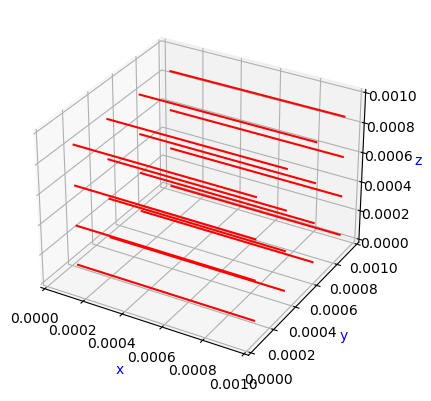
\includegraphics[width=3cm]{figures/J0/I10nr101lablength0.001tmax0.1J0Gamma10000000000.0mass3.58e-25len5e-05n1vel(0.01, 0, 0, 0, 0)swarmnum4norotFalsenosynFalse}}}
            \qquad
            \subfloat[\centering \(J = 0\), \(n =
            1\), \(m = 3.58\times 10^{-28}\) kg]{{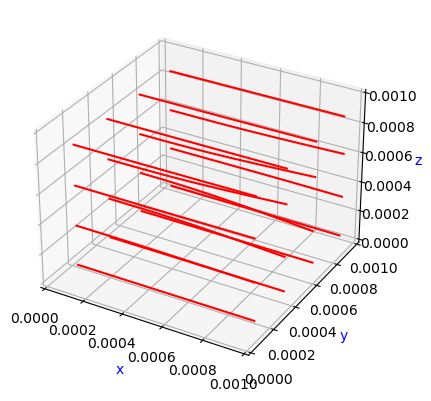
\includegraphics[width=3cm]{figures/J0/I10nr101lablength0.001tmax0.1J0Gamma10000000000.0mass3.58e-28len5e-05n1vel(0.01, 0, 0, 0, 0)swarmnum4norotFalsenosynFalse}}}
            \qquad
            \subfloat[\centering \(J = 0\), \(n =
            1\), \(m = 3.58\times 10^{-29}\) kg]{{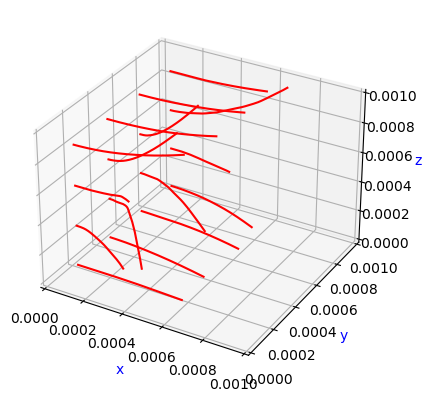
\includegraphics[width=3cm]{figures/J0/I10nr101lablength0.001tmax0.1J0Gamma10000000000.0mass3.58e-29len5e-05n1vel(0.01, 0, 0, 0, 0)swarmnum4norotFalsenosynFalse}}}
            \caption{\centering Three different masses for \(n = 1\), \(J = 0\)}%
        \end{figure}
\end{frame}
\subsection{The high energy state}
\begin{frame}
        \frametitle{The high energy state I}
		\begin{figure}[h]
		    \centering
		    \subfloat[\centering With synthetic fields in red,
		    without in blue]{{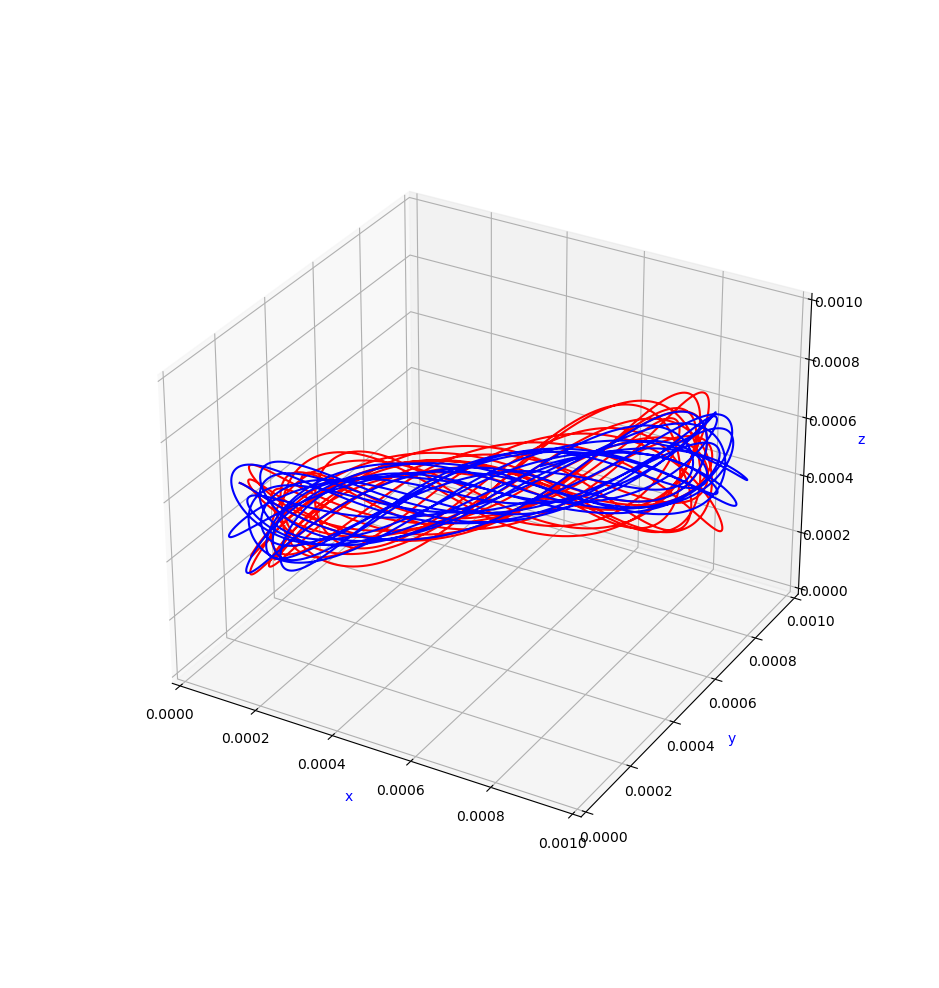
\includegraphics[width=3.5cm]{figures/n2m-25/(0,2)-comp1}}}
		    \qquad
		    \subfloat[\centering Without synthetic magnetic field in green,
		    without synthetic scalar field in yellow]{{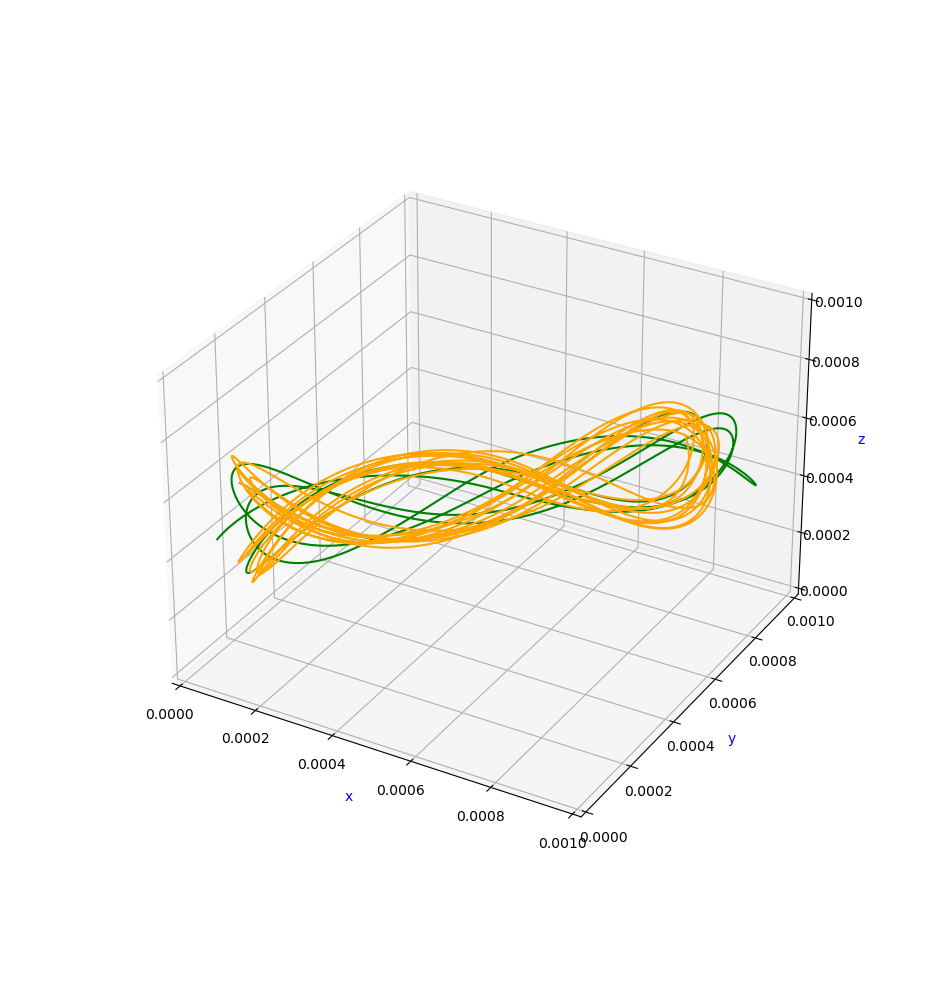
\includegraphics[width=3.5cm]{figures/n2m-25/(0,2)-comp2}}}
		    \qquad
		    \subfloat[\centering Without any synthetic fields in blue, without synthetic
            magnetic field in green]{{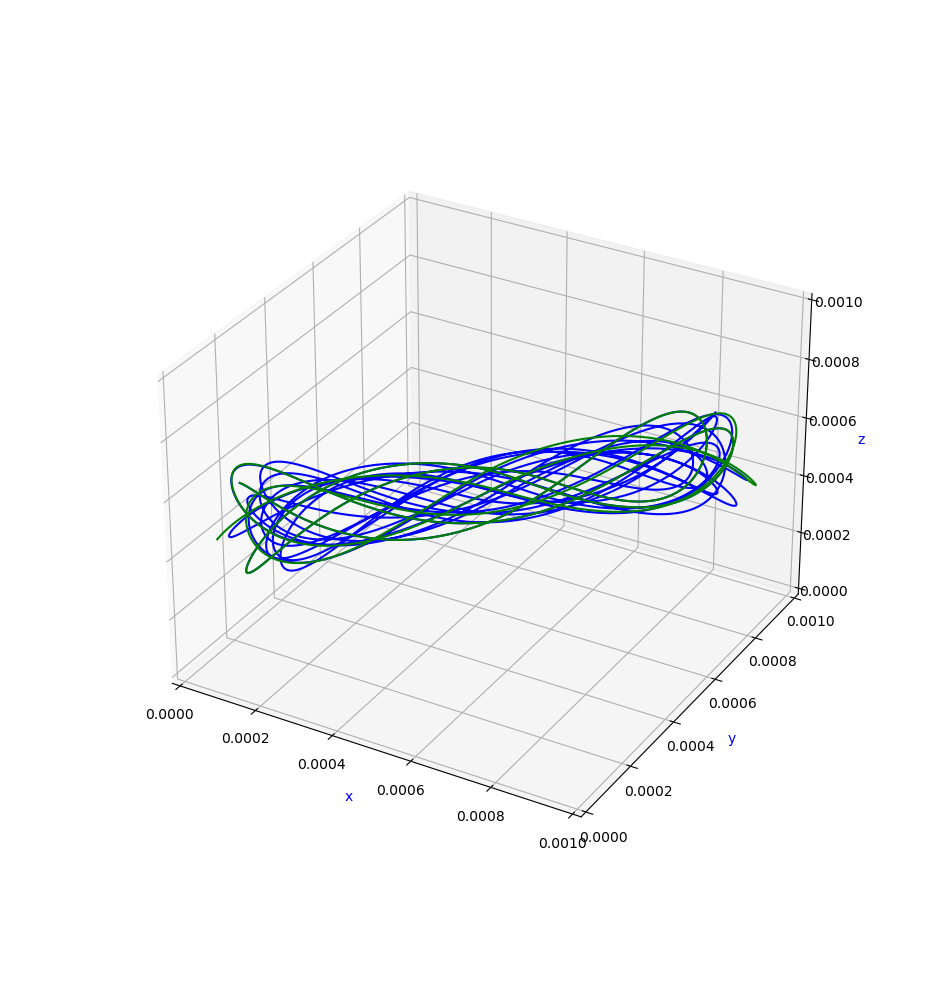
\includegraphics[width=3.5cm]{figures/n2m-25/(0,2)-comp3}}}
		\end{figure}
        \begin{itemize}
                \item A direct comparison between different fields with \(m= 3.58\times
                        10^{-25}\) kg.
        \end{itemize}
\end{frame}
\begin{frame}
        \frametitle{The high energy state II}
		\begin{figure}[h]
		    \centering
		    \subfloat[\centering With synthetic fields in red,
		    without in blue]{{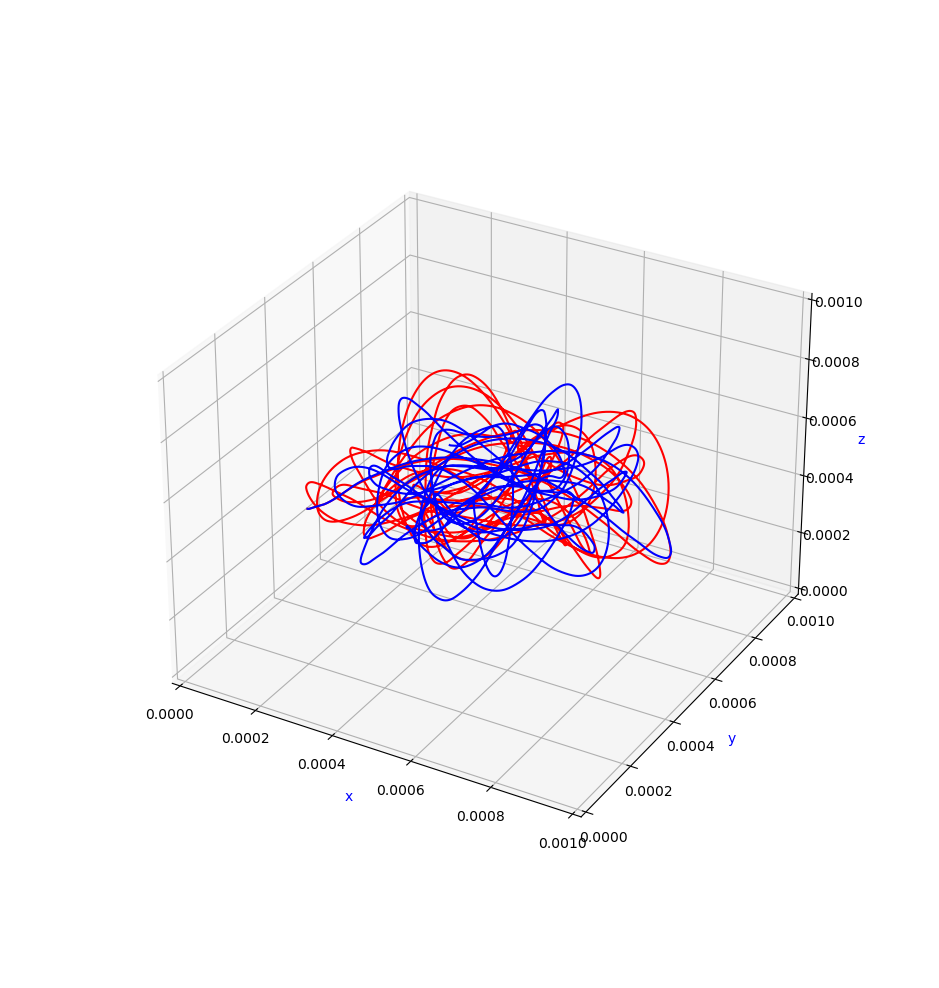
\includegraphics[width=4cm]{figures/n2m-27/(1,1)-comp1}}}
		    \qquad
		    \subfloat[\centering Without synthetic magnetic field in green,
		    without synthetic scalar field in yellow]{{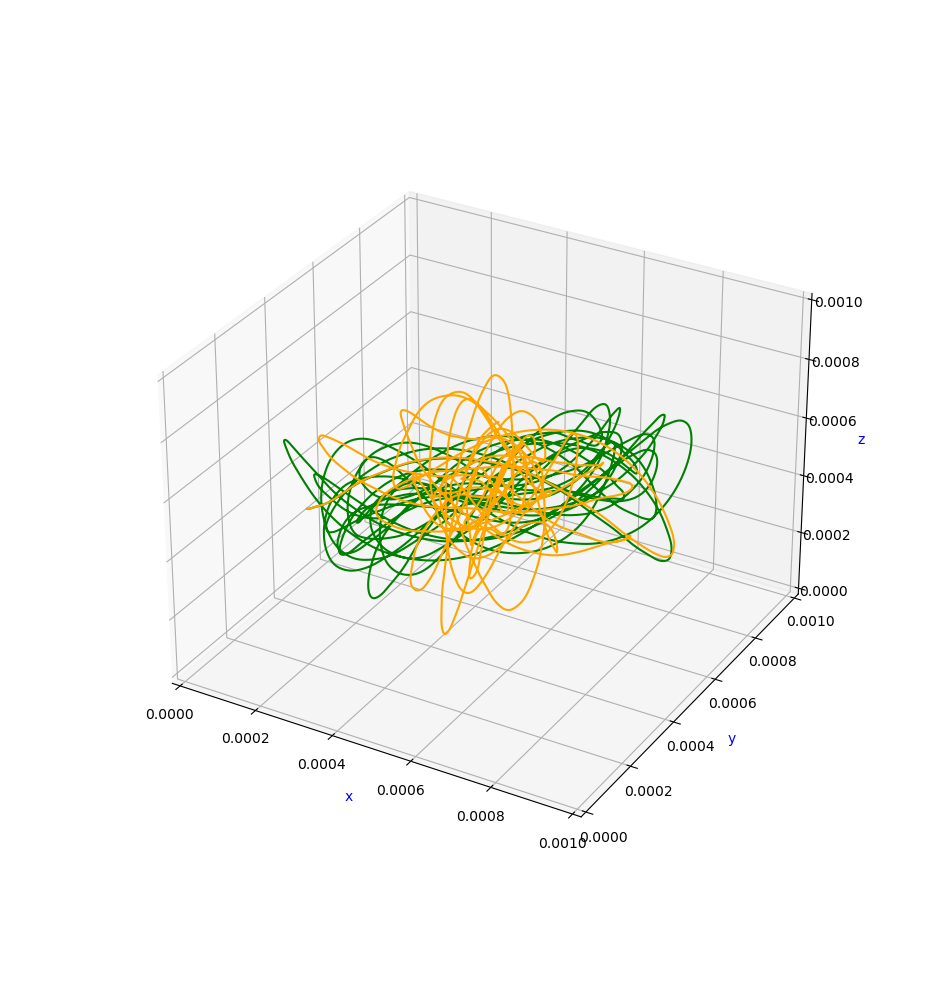
\includegraphics[width=4cm]{figures/n2m-27/(1,1)-comp2}}}
            \begin{itemize}
                    \item The same procedure for \(m = 3.58\times 10^{-27}\) kg and
                            \(\gamma = 10^{8}\) J/\(\hbar{}\).
            \end{itemize}
		\end{figure}
\end{frame}
\begin{frame}
		\begin{figure}[h]
		    \centering
		    \subfloat{{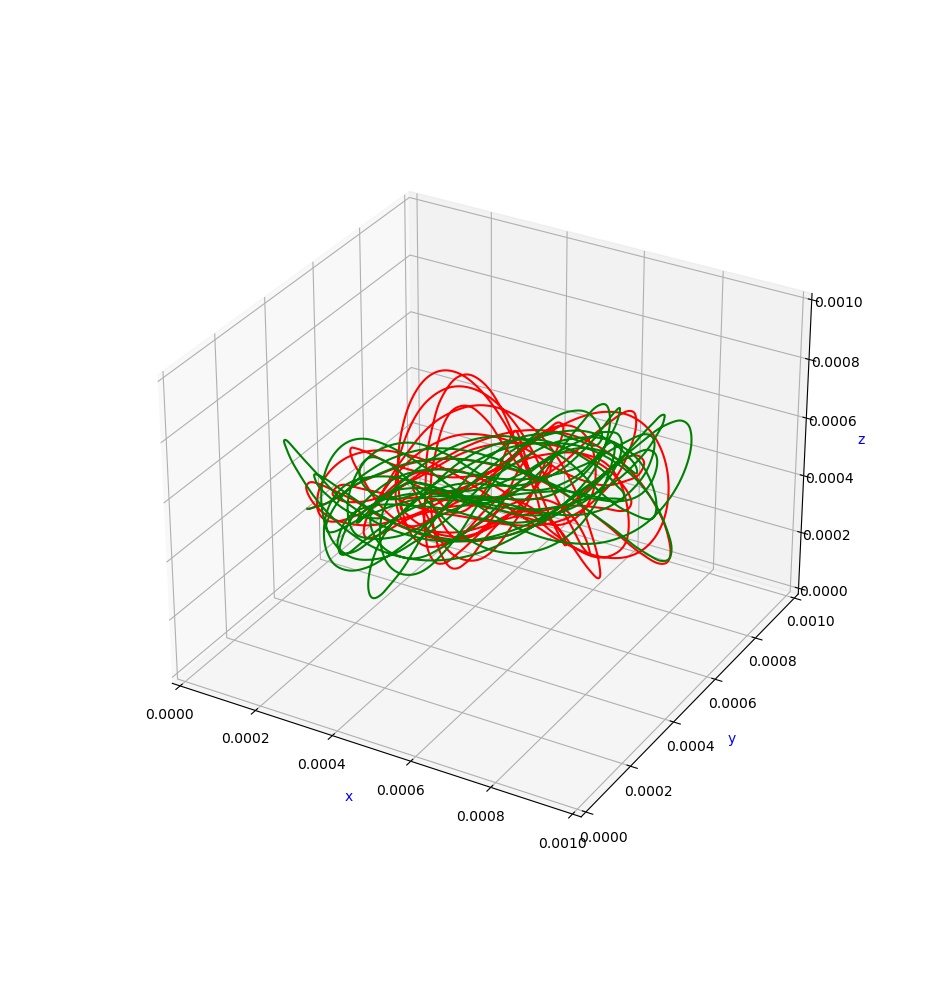
\includegraphics[width=4cm]{figures/n2m-27/(1,1)-comp3}}}
		    \qquad
		    \subfloat{{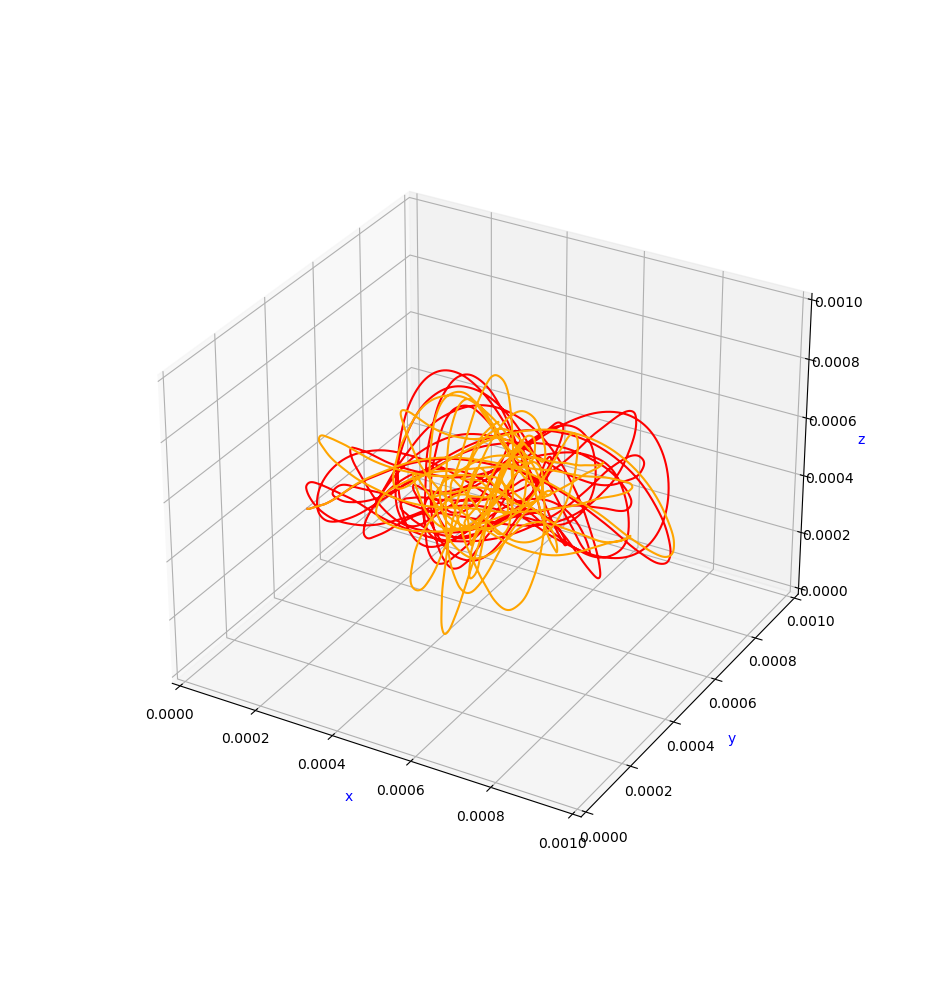
\includegraphics[width=4cm]{figures/n2m-27/(1,1)-comp4}}}
		    \qquad
		    \subfloat{{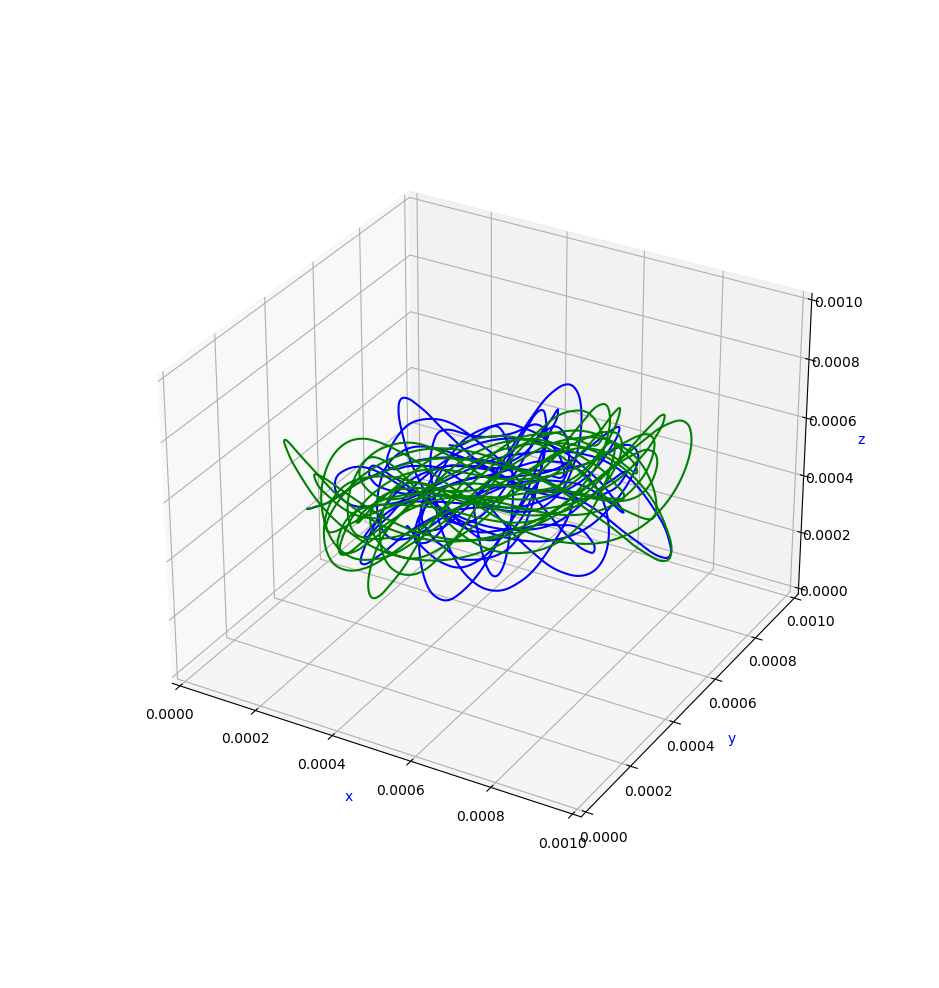
\includegraphics[width=4cm]{figures/n2m-27/(1,1)-comp5}}}
		    \qquad
		    \subfloat{{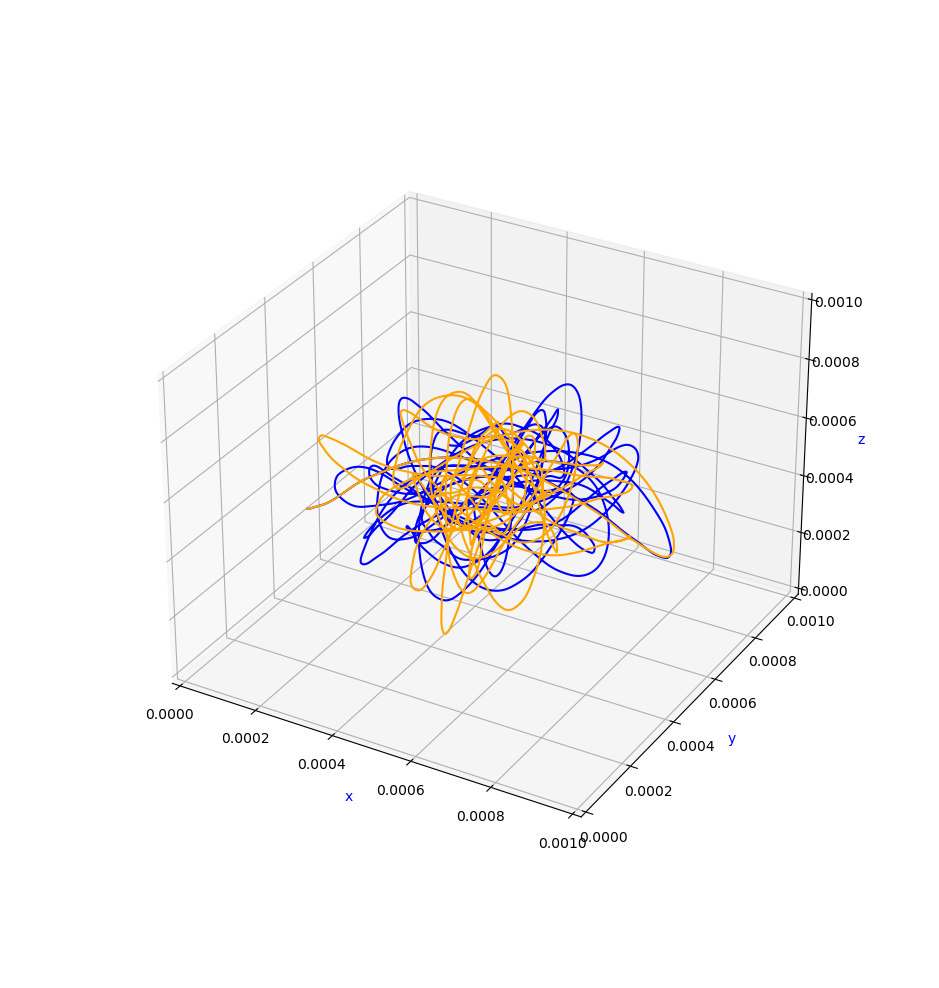
\includegraphics[width=4cm]{figures/n2m-27/(1,1)-comp6}}}
		\end{figure}
\end{frame}
\subsection{Conclusions}
\begin{frame}
        \frametitle{Conclusions}
        \begin{itemize}
                \item EOM and a script for their evaluation have been developed.
                \item The repulsive nature of the synthetic scalar field has been
                        demonstrated.
                \item Synthetic behaviour arising from monopolar fields play a significant
                        role for the time evolution of the selected system, for reasonable
                        masses.
                \item Mass is the main tool for increasing synthetic effects.
                \item Complication of the external field could also be viable but 
                        complicates interpretation of the result.
        \end{itemize}
\end{frame}
\begin{frame}
	\begin{figure}[h]
	        \centering
	        \begin{tikzpicture}
	                \draw[black]
	                        (-4, 0) node{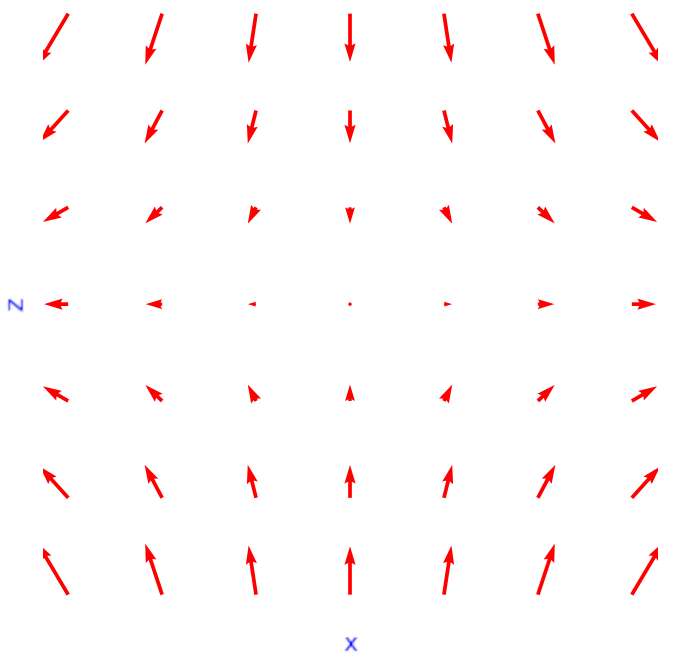
\includegraphics[width=0.3\textwidth]{figures/coilfield-e}};
	                \draw[black] (-3.9,-2.8) node{External field in real space.};
	                \draw[black, ->] (-1,0) to[out=30, in=150] (1,0);
	                \draw[black] (0,0.7) node{\(M\) };
	                \draw[black]
	                        (4, 0)node[yshift=0.4]{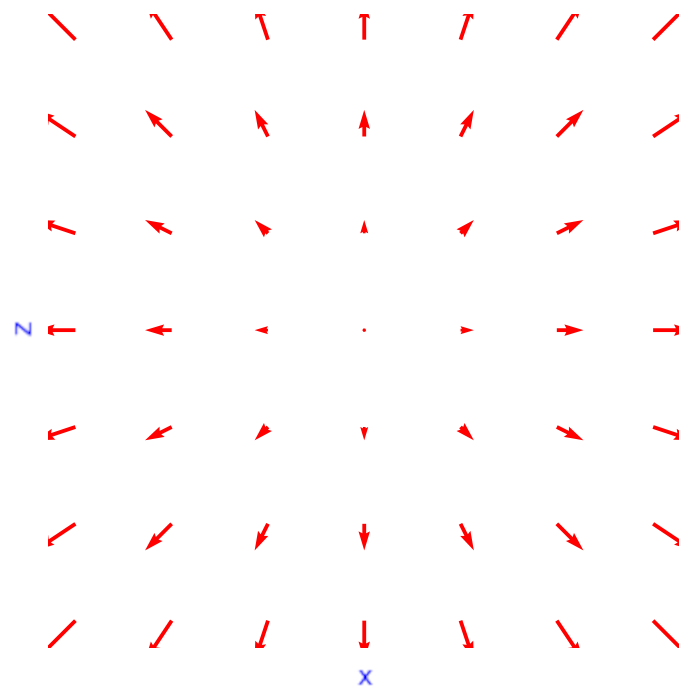
\includegraphics[width=0.29\textwidth]{figures/idealfield-e}};
	                \draw[black] (4.1,-2.8) node{External field in parameter space.};
	        \end{tikzpicture}
	        \caption{\centering An illustration of the map \(M\) between real space and parameter space,
	        which must map every point of external field \(\va{b}\) to the parameter space
	point with the same external field \(\va{b}\). The planes shown are the \(xz\)-planes
	through the zero-field centre point of the lab and the origin, respectively.}
	        \label{fig:fieldcompare}
	\end{figure}
\end{frame}
\section{The next steps}
\begin{frame}
        \frametitle{The next steps}
        \begin{itemize}
                \item How would we precisely separate and interpret the synthetic action as
                        a monopolar one? Technical difficulties need be addressed.
                \item The performance of the simulations are a limiting factor, optimize
                        or run on better hardware (UPPMAX).
                \item Realising the system could perhaps be done, how would such a setup
                        look?
        \end{itemize}
\end{frame}
\begin{frame}
        \frametitle{Questions?}
        \begin{center}
        
\includegraphics[width=0.3\textwidth]{qr-code}
        \end{center}
\blfootnote{Presentation template by \textit{Frederic Haziza},
        \url{http://www.it.uu.se/katalog/daz/uppsala_beamer}}
\end{frame}
\end{document}
